% THIS IS SIGPROC-SP.TEX - VERSION 3.1
% WORKS WITH V3.2SP OF ACM_PROC_ARTICLE-SP.CLS
% APRIL 2009
%
% It is an example file showing how to use the 'acm_proc_article-sp.cls' V3.2SP
% LaTeX2e document class file for Conference Proceedings submissions.
% ----------------------------------------------------------------------------------------------------------------
% This .tex file (and associated .cls V3.2SP) *DOES NOT* produce:
%       1) The Permission Statement
%       2) The Conference (location) Info information
%       3) The Copyright Line with ACM data
%       4) Page numbering
% ---------------------------------------------------------------------------------------------------------------
% It is an example which *does* use the .bib file (from which the .bbl file
% is produced).
% REMEMBER HOWEVER: After having produced the .bbl file,
% and prior to final submission,
% you need to 'insert'  your .bbl file into your source .tex file so as to provide
% ONE 'self-contained' source file.
%
% Questions regarding SIGS should be sent to
% Adrienne Griscti ---> griscti@acm.org
%
% Questions/suggestions regarding the guidelines, .tex and .cls files, etc. to
% Gerald Murray ---> murray@hq.acm.org
%
% For tracking purposes - this is V3.1SP - APRIL 2009

\documentclass{acm_proc_article-sp}

\usepackage[utf8]{inputenc}
\usepackage[brazilian]{babel}
\usepackage{color}
\usepackage{listings}

\newcommand{\todo}[1]{\textcolor[rgb]{1.00,0.00,0.00}{\bf \uppercase{#1}}}

\begin{document}

\title{Uma nova API para criação de videoconferências em dispositivos móveis Android}
%
% You need the command \numberofauthors to handle the 'placement
% and alignment' of the authors beneath the title.
%
% For aesthetic reasons, we recommend 'three authors at a time'
% i.e. three 'name/affiliation blocks' be placed beneath the title.
%
% NOTE: You are NOT restricted in how many 'rows' of
% "name/affiliations" may appear. We just ask that you restrict
% the number of 'columns' to three.
%
% Because of the available 'opening page real-estate'
% we ask you to refrain from putting more than six authors
% (two rows with three columns) beneath the article title.
% More than six makes the first-page appear very cluttered indeed.
%
% Use the \alignauthor commands to handle the names
% and affiliations for an 'aesthetic maximum' of six authors.
% Add names, affiliations, addresses for
% the seventh etc. author(s) as the argument for the
% \additionalauthors command.
% These 'additional authors' will be output/set for you
% without further effort on your part as the last section in
% the body of your article BEFORE References or any Appendices.

\numberofauthors{4} %  in this sample file, there are a *total*
% of EIGHT authors. SIX appear on the 'first-page' (for formatting
% reasons) and the remaining two appear in the \additionalauthors section.
%
\author{
% You can go ahead and credit any number of authors here,
% e.g. one 'row of three' or two rows (consisting of one row of three
% and a second row of one, two or three).
%
% The command \alignauthor (no curly braces needed) should
% precede each author name, affiliation/snail-mail address and
% e-mail address. Additionally, tag each line of
% affiliation/address with \affaddr, and tag the
% e-mail address with \email.
%
% 1st. author
\alignauthor
Giancarlo Rampanelli, 
Felipe Cecagno,
André Schulz,
Valter Roesler\\
       \affaddr{Laboratório do PRAV}\\
       \affaddr{Instituto de Informática}\\
       \affaddr{Universidade Federal do Rio Grande do Sul}\\
       \affaddr{Av. Bento Gonçalves, 9500 - Bloco IV, Prédio 72, Sala 220}\\
       \affaddr{Porto Alegre, Brasil}\\
       \email{\{grampanelli, fcecagno, aschulz, roesler\}@inf.ufrgs.br}
}
\date{15 de maio de 2011}

\maketitle
\begin{resumo}
  Este artigo tem o objetivo de apresentar uma nova estratégia para criação de videoconferências em dispositivos móveis com sistema operacional Android. Será apresentado um estudo sobre as classes multimídia padrão do kit de desenvolvimento de software do Android, detalhando as limitações que dificultam o desenvolvimento de sistemas multimídia em tempo real sem a utilização de bibliotecas externas. Várias soluções são comparadas, ressaltando prós e contras, e conduzindo a necessidade da utilização de uma nova estratégia, detalhada neste artigo, que é baseada principalmente em bibliotecas alternativas. A ideia proposta é então validada num sistema Android real, mostrando suas vantagens.
\end{resumo}

\begin{abstract}
  This article aims to present a strategy for implementation of real-time interactive multimedia systems on Android-powered mobile devices. We will present a study about the standard multimedia classes of Android’s software development kit, detailing the limitations that hinder the development of real time multimedia systems without using external libraries. Some alternative solutions proposed in previous works will be presented, highlighting pros and cons of each one, concluding with the contribution of this paper, a solution based primarily on alternative libraries.
\end{abstract}

% http://www.acm.org/about/class/ccs98-html
% A category with the (minimum) three required fields
\category{}{Peer-to-peer multimedia systems and streaming}{}
\category{}{Software development using multimedia techniques}{}
%\category{H.4}{Information Systems Applications}{Miscellaneous}

%\terms{Theory}

\keywords{Interação multimídia de tempo real, Vídeo, JNI}

\section{Introdução}

\todo{verificar se os autores ficarão dessa forma ou agrupados}

\todo{verificar categorias oficiais da acm}

\todo{verificar termos que serão utilizados}

\todo{este é um capítulo que provavelmente iremos reduzir para caber tudo em oito páginas}

Um sistema que permite que uma pessoa comunique-se, ao vivo, com uma ou mais
pessoas, cada qual em sua máquina, através da transmissão da sua fala (capturada pelo microfone) e da sua imagem em forma de vídeo (capturada pela câmera), ao mesmo tempo em que escuta e visualiza os outros participantes, representa um sistema de transmissão de vídeo interativo em tempo real. Tais sistemas são complexos de serem desenvolvidos, já que, além da necessidade do áudio e do vídeo serem transmitidos, recebidos e exibidos de forma contínua por todos os participantes, é preciso que essa transmissão ocorra com um baixíssimo atraso: se o intervalo de tempo entre o instante da captura do áudio e do vídeo e o instante da sua exibição nas máquinas dos outros participantes for maior que 400 milissegundos, por exemplo, o resultado pode ser uma interação altamente frustrante \cite{kurose_2001}.

É um desafio desenvolver com qualidade tais sistemas pois as redes atuais, em geral, suportam apenas uma pequena taxa de bit/s. O desafio se torna ainda maior na área dos dispositivos móveis, que, além de terem hardware limitado, que torna a tarefa da decodificação e da exibição do vídeo menos eficiente, também têm limitações de rede, pois costumam utilizar 3G ou Internet sem fio, ambos suscetíveis a alta perda de pacotes e, na maioria das vezes, a baixas velocidades \cite{huynh-thu_2008}.

Um exemplo de utilização dessa técnica se dá em videoconferências, que correspondem a reuniões remotas nas quais os participantes podem, por vídeo, interagir e colaborar com o propósito da reunião. Mesmo estando, cada um, em lugares diferentes, a utilização do vídeo lhes sugere que todos estão presentes em uma mesma sala, aumentando a efetividade da colaboração em comparação a uma reunião remota por texto ou por voz apenas.

Um vídeo interativo pode ser dividido, basicamente, em dois módulos:
\begin{itemize}
 \item Um módulo para gerenciar o lado da origem, dividido em 3 sub-módulos:
 \begin{itemize}
  \item Um sub-módulo para capturar quadros de áudio e de vídeo não comprimidos do microfone e da câmera, respectivamente;
  \item Um sub-módulo para codificar os quadros de áudio e de vídeo;
  \item Um sub-módulo para enviar pela rede os dados codificados;
 \end{itemize}
 \item Um módulo para gerenciar o lado do destino, dividido em 3 sub-módulos:
 \begin{itemize}
  \item Um sub-módulo para receber pela rede dados de áudio e de vídeo codificados;
  \item Um sub-módulo para decodificar os dados;
  \item Um sub-módulo para renderizar os quadros de áudio e de vídeo decodificados.
 \end{itemize}
\end{itemize}

Neste trabalho iremos apresentar uma nova estratégia para criação de videoconferências em dispositivos móveis com sistema operacional Android.

\section{Análise da SDK do Android para multimídia}

Android é um sistema operacional de código aberto para dispositivos móveis, desenvolvido numa colaboração entre Google e outros membros da Open Handset Alliance, e baseado no núcleo do Linux. Em comparação aos outros sistemas operacionais para smartphones existentes, o Android é caracterizado por aplicações de vídeo mais simples. Isso se deve às limitações das APIs fornecidas pelo Android para programação de vídeo e, alternativamente, à grande complexidade para criar tais aplicativos sem a utilização dessas APIs. A dificuldade de se encontrar bons aplicativos de vídeo para Android se torna ainda mais marcante na área de vídeo interativo.

Aplicativos para Android são escritos na linguagem de programação Java e executam sobre a máquina virtual Dalvik. O desenvolvimento de aplicativos é feito com o kit de desenvolvimento de software para Android (Android SDK). Esse kit fornece diversas ferramentas úteis (como depuradores de código, emuladores e APIs) além de oferecer plataformas que permitem a compilação de aplicativos \cite{ableson_2009}.

Considerando os dois módulos de um sistema de interação por vídeo descritos anteriormente, as classes fornecidas pelo Android que têm utilidade para cada um desses módulos são:
\begin{itemize}
 \item para o módulo de origem: MediaRecorder, Camera e AudioRecord;
 \item para o módulo de destino: MediaPlayer e AudioTrack.
\end{itemize}

Existem outras classes relacionadas, porém estas apresentam pequenas extensões ou encapsulamentos das classes acima, sem importância para este trabalho. Também existem classes relacionadas ao envio e recebimento de dados genéricos pela rede que poderiam ser utilizadas em conjunto com as classes acima. A seguir as classes supracitadas serão detalhadas, e com base nas características de cada uma serão apresentadas estratégias de desenvolvimento de um sistema de vídeo interativo bem como suas limitações.

\subsection{Classe MediaRecorder}
A classe MediaRecorder realiza a captura de áudio e de vídeo (a partir do microfone e da câmera, respectivamente) e codifica-os utilizando o hardware do aparelho. Os dados codificados podem ser salvos encapsulados em um arquivo, ou podem ser transmitidos pela rede com a utilização de sockets. A classe também pode exibir um preview da captura para o usuário local.

A utilização do MediaRecorder acontece da seguinte forma:
\begin{enumerate}
 \item Declarar uma instância da classe
  \begin{verbatim}
MediaRecorder mMediaRecorder = new MediaRecorder();
  \end{verbatim}
 \item Escolher se as fontes de áudio e vídeo:
  \begin{verbatim}
mMediaRecorder.setAudioSource(<fonte de áudio>);
mMediaRecorder.setVideoSource(<fonte de vídeo>);
  \end{verbatim}
 \item Escolher o destino (arquivo ou socket)
  \begin{verbatim}
mMediaRecorder.setOutputFile(<destino>);
  \end{verbatim}
 \item Iniciar a captura:
  \begin{verbatim}
mMediaRecorder.prepare();
mMediaRecorder.start();
  \end{verbatim}
 \item Exibir o preview da captura:
  \begin{verbatim}
mMediaRecorder.setPreviewDisplay(<superfície local>);
  \end{verbatim}
\end{enumerate}

Portanto, a classe pode ser utilizada de duas formas diferentes: salvando em um arquivo ou utilizando um socket. Além de não prover um mecanismo de acesso direto aos dados capturados, também não há como acessar os dados codificados, impossibilitando o encapsulamento dos mesmos em um protocolo de aplicação antes de enviá-los através do socket, por exemplo. 

\subsection{Classe Camera}
A classe Camera realiza a captura de vídeo (a partir da câmera) e pode exibir um preview local da captura para o usuário. Ela pode ser utilizada de duas formas: para tirar fotos (ou seja, salvar um quadro da captura, codificando-o e encapsulado-o em um arquivo) ou para instalar um callback que é chamado a cada frame capturado e que recebe os dados não codificados do frame capturado.

\lstset{language=Java,captionpos=b,tabsize=3,frame=lines,keywordstyle=\color{blue},commentstyle=\color{darkgreen},stringstyle=\color{red},numbers=left,numberstyle=\tiny,numbersep=5pt,breaklines=true,showstringspaces=false,basicstyle=\scriptsize,emph={label}}

Basicamente, as etapas necessárias são as seguintes:
\begin{enumerate}
 \item Obter acesso à câmera:
%  \begin{lstlisting}
%Camera mCamera = Camera.open();
%  \end{lstlisting}
  \begin{verbatim}
Camera mCamera = Camera.open();
  \end{verbatim}
 \item Escolher a superfície de preview:
  \begin{verbatim}
mCamera.setPreviewDisplay(<superfície local>);
  \end{verbatim}
 \item Instalar o callback (opcional):
  \begin{verbatim}
mCamera.setPreviewCallback(<contexto>);
  \end{verbatim}
 \item Iniciar a captura:
  \begin{verbatim}
mCamera.startPreview();
  \end{verbatim}
 \item Tirar foto (opcional):
  \begin{verbatim}
takePicture(<Camera.ShutterCallback>,
    <Camera.PictureCallback>,
    <Camera.PictureCallback>);
  \end{verbatim}
 \item Obter os dados não codificados do frame capturado (opcional):
  \begin{verbatim}
@Override
public void onPreviewFrame (byte[] data, 
    Camera camera){}
  \end{verbatim}
\end{enumerate}


\subsection{Classe AudioRecord}
A classe AudioRecord realiza a captura de áudio (a partir do microfone) e, enquanto captura, escreve os dados não codificados em um buffer principal. Esses dados podem ser transferidos para um buffer secundário sempre que se desejar, para que possam ser utilizados.

Basicamente, as etapas necessárias são as seguintes:
\begin{enumerate}
 \item Declarar uma instância da classe:
  \begin{verbatim}
AudioRecord mAudioRecord = new AudioRecord(
    MediaRecorder.AudioSource.MIC, 
    <taxa de amostragem>,
    <numero de canais>,
    <bits por amostra>,
    <tamanho do buffer principal>);
  \end{verbatim}
 \item Iniciar a captura:
  \begin{verbatim}
mAudioRecord.startRecording();
  \end{verbatim}
 \item Transferir o conteúdo do buffer principal (quando desejado) para um buffer secundário:
  \begin{verbatim}
record.read(<buffer secundário>,
    <índice inicial do buffer secundário>,
    <número de bytes a transferir>);
  \end{verbatim}
\end{enumerate}

\subsection{Classe MediaPlayer}
A classe MediaPlayer fornece funções de alto nível para a exibição de vídeos. Basicamente, permite a escolha da origem do vídeo (arquivo local, servidor web ou streaming por RTSP), e faz o início da exibição~\cite{pro_android}. Dada a origem do vídeo, a classe realiza a decodificação do áudio e do vídeo em hardware e os renderiza.

Basicamente, as etapas necessárias são as seguintes:
\begin{enumerate}
 \item Declarar uma instância da classe:
  \begin{verbatim}
MediaPlayer mMediaPlayer = new MediaPlayer();
  \end{verbatim}
 \item Escolher a origem do vídeo:
  \begin{verbatim}
mMediaPlayer.setDataSource(<origem do vídeo>);
  \end{verbatim}
 \item Iniciar o processo de recebimento (caso a origem do vídeo seja remota), decodificação e renderização:
  \begin{verbatim}
mMediaPlayer.prepare();
mMediaPlayer.start();
  \end{verbatim}
\end{enumerate}

\subsection{Classe AudioTrack}
A classe AudioTrack serve para renderizar áudio. Sempre que se desejar renderizar áudio com ela, deve-se transferir os dados de áudio não codificados de um buffer secundário para o buffer principal da classe.

Basicamente, as etapas necessárias são as seguintes:
\begin{enumerate}
 \item Declarar uma instância da classe:
  \begin{verbatim}
mAudioTrack = new AudioTrack(<tipo de stream>,
    <taxa de amostragem>,
    <numero de canais>,
    <bits por amostra>,
    <tamanho do buffer principal>,
    <modo (estático ou stream)>);
  \end{verbatim}
 \item Caso o modo utilizado seja o stream, chamar o método play():
  \begin{verbatim}
mAudioTrack.play();
  \end{verbatim}
  Nada será renderizado pois o buffer principal está vazio.
 \item Transferir o conteúdo do buffer secundário (quando desejado) para o buffer principal:
  \begin{verbatim}
mAudioTrack.write(<buffer secundario>,
    <índice inicial do buffer secundário>,
    <número de bytes a transferir>);
  \end{verbatim}
Caso o modo utilizado seja o stream, cada vez que o buffer principal receber novos dados, eles serão reproduzidos sem a necessidade de chamar o método play().
 \item Caso o modo utilizado seja o estático, chamar o método play() para renderizar os dados (quando desejado):
  \begin{verbatim}
mAudioTrack.play();
  \end{verbatim}
\end{enumerate}

\section{Estratégias para STVITR com as classes padrão}

\subsection{Estratégia 1}
É a técnica implementada em \todo{trab alemao}.

\subsubsection{Do lado da origem}

Esta estratégia consiste em iniciar uma captura de áudio e de vídeo com a classe MediaRecorder passando como parâmetro ao método setOutputFile um descritor de arquivo local (ex: /sdcard/temp0.3gp) e finalizar a captura após um período curto (ex: 2 segundos). Os dados codificados do arquivo que está sendo gerado vão sendo enviados desde o início da captura, utilizando uma classe do Android para transmissão genérica de dados. Seria muito mais simples passar como parâmetro ao método setOutputFile um socket localizado no destino. Assim os dados seriam enviados diretamente sem a utilização de arquivo local. No entanto, estamos querendo criar um sistema de STVITR utilizando apenas as classes padrão do Android, e a classe MediaPlayer (única capaz de reproduzir vídeo) reproduz apenas dados encapsulados ou com o container 3GPP ou com o container MPEG-4 (exceto quando é utilizado RTSP, que será abordado na estratégia seguinte). Ambos containers são muito similares, e só podem ser incluídos ao final da gravação do arquivo. A classe MediaRecorder, ao final da gravação de um arquivo, insere, no início do arquivo, o header e os metadados do container escolhido. O método, então, ao finalizar o período curto de gravação, abre o início do arquivo que foi gerado localmente e envia os headers e os metadados para o destino. Enquanto os headers e os metadados são enviados, repete-se todo o processo com outro arquivo local (ex: /sdcard/temp1.3gp) de mesma duração do anterior, e assim sucessivamente. \todo{dividir esse parágrafo em mais de um!}

\subsubsection{Do lado do destino}

O lado do destino vai recebendo os dados de áudio e vídeo que estão sendo enviados e vai armazenando-os em um arquivo. Quando, enfim, chegam o header e os metadados do container escolhido, eles são inseridos no início desse arquivo. Somente nesse instante a classe MediaPlayer pode reproduzí-los. O processo é repetido para cada arquivo curto capturado, mas os dados são armazenados em um arquivo diferente para não sobrescrever o que está sendo reproduzido pela classe MediaPlayer.

\subsubsection{Análise da estratégia}

Segundo \todo{trab alemao}, a classe MediaRecorder leva 1,3 segundos (em média) para ser inicializada. E não é possivel inicializar um novo MediaRecorder antes de finalizar o anterior. Logo, utilizando esta estratégia, ocorreriam períodos de 1,3 segundos em que não se poderia capturar nada. Do lado do destino, considerando apenas essa limitação, isso seria percebido como travamentos de 1,3 segundos no vídeo seguidos de saltos de 1,3 segundos na sua exibição. A classe MediaPlayer só pode ser inicializada quando o arquivo estiver pronto, e a demora na sua inicialização é, em média, 0,83 segundos.
supondo:

\begin{itemize}
 \item duração de cada captura = 2s.
 \item tempo para inicializar a classe MediaRecorder = 1.3s.
 \item tempo para inicializar a classe MediaPlayer = 0.9s.
 \item tempo para a classe MediaRecorder inserir os metadados no início do arquivo = 0.1s.
 \item tempo para o lado do destino inserir os metadados no início do arquivo = 0.1s.
 \item tempo para transmitir um pacote pela rede = 0.1s.
 \item t = 0s a 1.3s: lado da origem: Classe MediaRecorder é inicializada.
 \item t = 1.3s: lado da origem: a inicialização da Classe MediaRecorder está pronta e a captura inicia.
 \item t = 1.3s a 3.3s: lado da origem: o arquivo local “01origem” está sendo gerado e os dados úteis do vídeo estão sendo transmitidos.
 \item t = 1.4s: lado do destino: os primeiros pacotes começam a ser recebidos.
 \item t = 3.3s: lado da origem: a captura é finalizada.
 \item t = 3.4s: lado da origem: os metadados são inseridos pela classe MediaRecorder no início do arquivo local “01origem”. Em seguida o header e os metadados são enviados ao destino.
 \item t = 3.4s: lado do destino: todos os pacotes de áudio e vídeo já foram recebidos. Faltam o header e os metadados.
 \item t = 3.4s: lado da origem: a classe MediaRecorder é inicializada novamente.
 \item t = 3.5s: lado do destino: o header e os metadados são recebidos.
 \item t = 3.6s: destino: o header e os metadados são inseridos no início do arquivo “01destino”.
 \item t = 3.6s: destino: a classe MediaPlayer é inicializada.
 \item t = 4.5s: destino: a classe MediaPlayer começa a renderização do arquivo “01destino”. (atraso = 4.5 - 1.3 = 3.2s).
 \item t = 4.7s: origem: a inicialização da Classe MediaRecorder está pronta e a captura inicia.
 \item t = 4.7s a 6.7s: origem: o arquivo local “02origem” está sendo gerado e os dados úteis do vídeo estão sendo transmitidos.
 \item t = 4.8s: destino: os primeiros pacotes da nova captura começam a ser recebidos.
 \item t = 6.5s: destino: a classe MediaPlayer finaliza a renderização do arquivo “01destino”.
 \item t = 6.7s: origem: a captura é finalizada.
 \item t = 6.8s: lado da origem: os metadados são inseridos pela classe MediaRecorder no início do arquivo local “02origem”. Em seguida o header e os metadados são enviados ao destino.
 \item t = 6.8s: destino: todos os pacotes de áudio e vídeo já foram recebidos. Faltam o header e os metadados.
 \item t = 6.8s: origem: a classe MediaRecorder é inicializada novamente.
 \item t = 6.9s: destino: o header e os metadados são recebidos.
 \item t = 7.0s: destino: o header e os metadados são inseridos no início do arquivo “02destino”.
 \item t = 7,0s: destino: a classe MediaPlayer é inicializada.
 \item t = 7.9s: destino: a classe MediaPlayer começa a renderização do arquivo “02destino”. (atraso = 7.9 - 4.7 = 3.2s. Tempo sem exibição = 7.9 - 6.5 = 1.4s).
 \item t = 8.1s: origem: a inicialização da Classe MediaRecorder está pronta e a captura inicia.
 \item t = 8.1s a 10.1s: origem: o arquivo local “03origem” está sendo gerado e os dados úteis do vídeo estão sendo transmitidos.
 \item t = 8.2s: destino: os primeiros pacotes da nova captura começam a ser recebidos.
 \item t = 9.9s: destino: a classe MediaPlayer finaliza a renderização do arquivo “02destino”.
 \item t = 10.1s: origem: a captura é finalizada.
 \item t = 10.2s: lado da origem: os metadados são inseridos pela classe MediaRecorder no início do arquivo local “03origem”. Em seguida o header e os metadados são enviados ao destino.
 \item t = 10.2s: destino: todos os pacotes de áudio e vídeo já foram recebidos. Faltam o header e os metadados.
 \item t = 10.2s: origem: a classe MediaRecorder é inicializada novamente.
 \item t = 10.3s: destino: o header e os metadados são recebidos.
 \item t = 10.4s: destino: o header e os metadados são inseridos no início do arquivo “03destino”.
 \item t = 10.4s: destino: a classe MediaPlayer é inicializada.
 \item t = 11.3s: destino: a classe MediaPlayer começa a renderização do arquivo “03destino”. (atraso = 11.3 - 8.1 = 3.2s. Tempo sem exibição = 11.3 - 9.9 = 1.4s).
\end{itemize}

E assim por diante. \todo{talvez fosse melhor representar essa linha de tempo com uma imagem}

\todo{muito dado, na minha opinião. ficou muito longa essa parte. remover a linha do tempo e explicar em parágrafos a essência.}

Portanto, nessa simulação, o atraso é de 3.2 segundos. Além disso, ocorrem pausas de 1.4s a cada 2s de exibição do vídeo. Em um STVITR, o atraso não deve ultrapassar 400ms. Não existe uma norma para determinar a aceitabilidade pausas na exibição, mas é evidente que as pausas obtidas nesse método tornariam a comunicação altamente frustrante. O autor reconhece que a técnica não serve para STVITR, mas seu objetivo era identificar as limitações das APIs e propor a melhor aproximação possível de um STVITR. Segundo o autor, essa provavelmente é a técnica possível de ser implementada com as classes padrão do Android que mais se aproxima de um STVITR. No entanto, ele deixa claro que sempre podem surgir novas ideias. 

\subsection{Estratégia 2}
É a técnica implementada em \todo{sipdroid}.

Esta técnica utiliza a capacidade da classe MediaPlayer em reproduzir conteúdo ao vivo \todo{diferenciar conteúdo ao vivo de conteúdo em tempo real} utilizando o protocolo RTSP.

\subsubsection{Lado da origem}
A classe MediaRecorder é utilizada para capturar vídeo. O método setOutputFile recebe como parâmetro um descritor de arquivo obtido de um socket implementado pela classe LocalSocket do Android. Isso significa que os dados capturados não são salvos em um arquivo local, mas sim diretamente enviados para um socket. Os dados do socket são lidos e tratados para ficarem de acordo com o protocolo RTSP.

\subsubsection{Lado do destino}
A classe MediaPlayer é inicializada e o seu método setDataSource é setado para o endereço do stream RTSP.

\subsubsection{Análise do método}
O método acaba resultando em um sistema de vídeo ao vivo, e não em um STVITR, pois a implementação de RTSP do Android não serve para tempo real. Para provar isso, realizamos o seguinte teste :

\begin{enumerate}
 \item Capturamos vídeo com uma webcam conectada a um desktop utilizando o software VideoLAN .
 \item Direcionamos o fluxo para um servidor de streaming RTSP (Darwin Streaming Server) especificado por um arquivo SDP (Session Description Protocol).
 \item Recebemos o stream em um Motorola Milestone rodando Android 2.0.1 utilizando a API MediaPlayer.
\end{enumerate}

O atraso obtido foi de 10 segundos. Recebendo o mesmo stream no próprio VLC (ao invés de recebê-lo no Android), o atraso foi de 1 segundo.	 	 	

Também fizemos uma comparação do RTSP do Android com o RTSP do VideoLAN utilizando diversos links RTSP encontrados na Internet. Para todos eles, o vídeo exibido no Android foi exibido com um atraso entre 2 e 20 segundos após o mesmo vídeo sendo exibido no VídeoLAN.

Comparado ao método anterior, neste método não ocorrem pausas na exibição. Porém, segundo os testes de desempenho realizados com a classe MediaPlayer, o atraso é maior que o do método anterior, devido ao baixo desempenho do RTSP utilizado juntamente com a classe MediaPlayer do Android.

\subsection{Estratégia 3}

Ao invés de utilizar a classe MediaRecorder para capturar, utilizar as classes Camera e AudioRecord. Com ambas as classes é possível se obter os dados não codificados dos quadros de vídeo e de áudio capturados. No entanto, não há nenhuma classe padrão do android que receba como parâmetro um quadro não codificado e que codifique-o. E quadros não codificados são grandes demais para serem transmitidos pela rede em tempo viável para STVITR. Poderia ser implementado um codificador/decodificador em Java. No entanto, a tarefa da codificação/decodificação é extremamente custosa computacionalmente, além de ser muito complexa de ser desenvolvida. Implementar uma tarefa custosa em uma linguagem que roda em máquina virtual que, por sua vez, roda em um dispositivo de baixo poder computacional, seria pouco eficiente. Além disso, mesmo que fosse possível codificar os quadros em Java, enviá-los ao destino e decodificá-los em Java em tempo viável para STVITR, não haveria como reproduzí-los utilizando as classes padrão do Android, visto que nenhuma delas tem a capacidade de receber como parâmetros quadros decodificados. Logo, esta estratégia não é possível.

\subsection{Estratégia 4}

\subsubsection{Lado da origem}

Utilizar a função de foto da classe câmera, que retorna um frame codificado em JPEG, e enviar cada frame pela rede para o destino.

\subsubsection{Lado do destino}

Receber cada frame e exibí-lo com alguma classe padrão do Android que decodifique e exiba imagens JPEG.

\subsubsection{Análise da estratégia}

Codecs de vídeo são mais eficazes que o codec de imagens JPEG, visto que um vídeo é um conjunto de imagens relacionadas entre si, e a compressão é realizada com base na relação entre essas imagens. Um codec JPEG apenas comprime uma imagem sem relacioná-la com nenhuma outra, portanto tem menos poder de compressão. Além disso, a função foto do Android não foi projetada para este uso e é pouco eficiente. Um dos motivos é que quando a função foto é chamada, o preview do vídeo capturado é interrompido. Para tirar uma nova foto é preciso reiniciar o preview. O método em si não foi testado, mas certamente a taxa de frames e o atraso obtidos não chegariam perto do recomendado para STVITR. Outro problema dessa estratégia é não ter um correspondente para o áudio. Somente o vídeo seria transmitido.

\subsection{Estratégia 5}
Como o Android é de código aberto, essa estratégia seria copiar as libraries nativas (C/C++) internas (privadas) ao sistema operacional que interagem com as classes java MediaPlayer e MediaRecorder e com o hardware dos aparelhos e colá-las no em um novo projeto. Em seguida, compilaríamos essas libraries dentro do nosso projeto, com a utilização da NDK \todo{explicar o que é a ndk}. Desse modo, teríamos acesso aos quadros codificados/decodificados pelo hardware e, desse modo, poderíamos utilizar alguma classe genérica de transmissão de dados do Android para realizar a transmissão/recepção desses quadros. Assim, a implementação ficaria desta forma:

Captura: câmera e microfone seriam acessados diretamente pelo C++, utilizando as libraries privadas do android correspondentes.

Codificação: em hardware, utilizando as libraries privadas do android correspondentes.

Transmissão: alguma classe padrão do Android para transmissão genérica de dados.

Recepção: alguma classe padrão do Android para transmissão genérica de dados.

Decodificação: em hardware, utilizando as libraries privadas do android correspondentes.

Renderização: display e alto falante seriam acessados diretamente pelo C++, utilizando as libraries privadas do android correspondentes.

Esta seria a solução mais eficiente possível, visto que todas as tarefas pesadas seriam realizadas em hardware, e os quadros trafegariam pela rede comprimidos. Contudo, como as bibliotecas nativas interagem com o resto do Android, e o sistema operacional muda muito a cada nova versão (e muda a cada modelo de aparelho também, mesmo dentro de uma mesma versão), haveria probabilidade de 50\% \todo{segundo desenvolvedor do android, apresentar fonte} do aplicativo deixar de funcionar em diferentes versões do Android ou funcionar apenas no modelo de aparelho cujo código utilizamos, e a manutenção para fazê-lo voltar a funcionar ou para que funcione em múltiplos aparelhos com certeza seria inviável em termos de complexidade. Por esses motivos, tal uso das bibliotecas privadas do Android não deve ser feito, segundo os desenvolvedores do Android. Além disso, com essa solução estaríamos limitados a utilizar os codecs suportados por padrão pelos aparelhos android. Por todos esses motivos, descartamos essa alternativa.

\section{Solução adotada}

Pela análise acima, pode-se perceber que não foi possível contruir um STVITR utilizando-se apenas as classes padrão do Android. É claro que novas idéias podem surgir. A solução adotada baseia-se em algumas das classes padrão do Android apresentadas, mas sua parte principal é focada em implementações independentes.

A solução consiste em:

\subsection{Lado da origem}
\begin{enumerate}
 \item Utilizar a classe Camera para capturar os quadros de vídeo e instalar um callback que receba cada frame não codificado obtido da captura. Com o auxilio dessa API, nós setamos os parâmetros de captura desejados (resolução, quadros/s, etc) e enviamos cada frame capturado no formato YUV420SP (também conhecido como NV21, que é o único formato de captura suportado por todos os aparelhos Android) para o C++. A JNI \todo{explicar o que é a JNI} é utilizada para passar os frames do Java para o C++.
Um detalhe que convém citar é a utilização de Java reflection \todo{explicar o que é java reflection} para que se possa utilizar a função setPreviewCallbackWithBuffer em versões do android anteriores a 2.2, quase dobrando a taxa de frames em comparação ao método setPreviewCallback, visto que essa função evita que o GC (garbage collector do android) interrompa o programa a cada frame.
 \item Utilizar a classe AudioRecord para capturar os quadros de áudio, e obter os quadros não codificados da captura. Para isso desenvolvemos uma classe em Java que faz uso da classe AudioRecord, e captura o audio do microfone. Cada frame capturado é enviado ao C++ no formato RAW (PCM) com a utilização da JNI.
 \item Como o Android roda sobre um kernel Linux (FU et al., 2010), foi possível compilar o ffmpeg \todo{explicar o que é o ffmpeg} em C (com a NDK) adaptado para o Android. Desse modo, é possível codificar cada quadro de forma mais eficiente que em um codificador Java. No entanto, a implementação de diversos codecs de vídeo importantes fornecida pelo ffmpeg requer que o quadro decodificado de entrada esteja no formato YUV420P. Nesses casos, antes de codificar o quadro, é preciso convertê-lo de YUV420SP para YUV420P, numa função implementada por nós.
 \item Enviar os frames codificados para o destino utilizando a implementação de sockets do C/C++. (Poderia-se passar os quadros codificados para o Java e enviá-los com alguma classe padrão do Android, mas a tarefa de passar os quadros com a JNI é custosa e complexa de ser implementada).
\end{enumerate}

\subsection{Lado do destino}
\begin{enumerate}
 \item Receber os quadros com a implementação de sockets do C/C++. (Igualmente poderia-se utilizar alguma classe padrão do Android, mas, pelo mesmo motivo citado no item Anterior, não é o mais indicado).
 \item Decodificar os quadros de áudio e de vídeo com o ffmpeg em C/C++ para o formato RGB. Para os casos em que o ffmpeg apenas decodifica para YUV420P, criamos uma função que converte de YUV420P para RGB.
 \item Não há como acessar o alto falante e para renderizar os quadros de áudio diretamente do C++. A solução encontrada é passar os quadros de áudio decodificados para a classe AudioTrack utilizando a JNI. Desse modo, eles são reproduzidos. A API AudioTrack toca frames de audio que são entregues a ela no formato RAW (PCM). Para enviarmos os frames de áudio do C++ para o Java, primeiramente tentamos chamar uma função Java a partir do C++ utilizando a JNI, passando como parâmetro o frame, que seria a solução mais simples. No entanto, esta solução ativa o Garbage collector a cada frame, o que causa uma enorme queda no desempenho, logo essa alternativa foi descartada. A alternativa que implementamos para evitar o GC foi utilizar uma técnica da JNI um pouco mais trabalhosa. Em resumo, essa técnica consiste na criação de um array em Java que representa um frame e de um array em C++ que também representa um frame. Em seguida, com chamadas a algumas funções da JNI, associamos os dois arrays para a mesma posição de memória para que eles sejam tratados como se fossem um só. Assim, cada vez que se atualiza o array do C++ com os dados do novo frame decodificado, essa atualização é automaticamente propagada ao array do java, sem que seja feita nenhuma cópia e nenhuma alocação de memoria adicional, resultando na solução mais eficiente que encontramos para renderizar o áudio.
 \item Não há como acessar o display para renderizar os quadros de vídeo diretamente do C++. Também não há alguma classe Java que receba como parâmetros quadros decodificados e renderize-os. A solução encontrada foi renderizar os quadros de vídeo com OpenGL ES \todo{explicar o que é opengl es} em C++, desenhando um retângulo com as dimensões desejadas e aplicando o frame de vídeo decodificado como textura RGB ao retângulo. No entanto, para que a renderização seja exibida no display, é necessário que a função de renderização do C++ seja chamada de dentro do método onDrawFrame da classe GLSurfaceView.Renderer do Java e retorne para esse método a cada frame.
\end{enumerate}

Outro detalhe importante, caso o frame decodificado esteja numa resolução, e se queira renderizá-lo em outra, verificamos que realizando esse redimensionamento com o ffmpeg é mais lento que com o OpenGL ES. Ainda assim, caso a versão do OpenGL ES do aparelho utilizado seja a 1.0, o redimensionamento é feito em software. Caso seja 1.1 em diante, o redimensionamento é feito em hardware. Outro detalhe: algumas versões do OpenGL ES suportam apenas texturas sobre retângulos de resolução cujas dimensões são potência de 2. Para poder desenhar o vídeo em qualquer resolução, criamos uma função que gera um retângulo com dimensões de potência de dois imediatamente maiores que as que irão ser utilizadas. Em seguida, a cada frame, aplica-se a textura com qualquer dimensão sobre parte desse retângulo.

Também realizamos cálculos considerando a resolução máxima da tela e a orientação do celular para que a exibição do vídeo esteja sempre centralizada na tela, independentemente da resolução e da orientação.

\section{Análise técnica}
\subsection{Teste 1}
Foi testada a decodificação e a exibição de um arquivo de vídeo local com a estratégia implementada em um dispositivo HTC Magic. Como resultado, para um vídeo de resolução 176x144, foram decodificados 227 quadros por segundo. A taxa de exibição obtida foi de 60 quadros por segundo (valor máximo suportado pelo aparelho).
\subsection{Teste 2}
Implementamos um aplicativo de videoconferência entre dispositivos móveis com a técnica apresentada. Para testar, realizamos uma conversa por vídeo com dois aparelhos Android caracterizados pela tabela~\ref{tabela_dispositivos}.
\begin{table*}
\centering
\caption{Dispositivos utilizados nos testes}
\label{tabela_dispositivos}
\begin{tabular}{|c|c|c|c|c|l} \hline
Modelo&Processador&Versao do Android&Resolução máxima&Versão do OpenGL ES\\ \hline
Motorola Milestone A853&500MHz&2.0.1&480x854&1.0\\ \hline
Samsung Galaxy S GT-I9000B&1000MHz&2.1-update1&480x800&1.1\\
\hline\end{tabular}
\end{table*}

Os parâmetros de codificação de vídeo utilizados no teste foram:
\begin{itemize}
 \item Resolução: 320x240
 \item Codec: MPEG-4
 \item Taxa de bits: 256Kbps
 \item GOP: 12
 \item Taxa de quadros: 15fps
\end{itemize}
Os parâmetros de codificação de áudio utilizados no teste foram:
\begin{itemize}
 \item Codec: MP2
 \item Taxa de bits: 64Kbps
 \item Frequência: 22050Hz
 \item Bits por amostra: 16
 \item Canais: 1
 \item Taxa de quadros: 19/s \todo{fps pra áudio?}
\end{itemize}
O vídeo era ampliado com o OpenGL ES para a resolução máxima do respectivo aparelho. A tabela~\ref{tabela_teste2} exibe os resultados do teste.
\begin{table*}
\centering
\caption{Resultados do Teste 2}
\label{tabela_teste2}
\begin{tabular}{|c|c|c|c|l} \hline
Dispositivo&Tipo de medida&Taxa de quadros&Tempo médio por quadro\\ \hline
Motorola&Captura do vídeo&15/s&1,16ms\\ \hline
Motorola&Captura do áudio&19/s&0,07ms\\ \hline
Samsung&Renderização do vídeo&14/s&2,88ms\\ \hline
Samsung&Renderização do áudio&18/s&19,62ms\\ \hline
Samsung&Captura do vídeo&15/s&0,72ms\\ \hline
Samsung&Captura do áudio&19/s&0,03ms\\ \hline
Motorola&Renderização do vídeo&15/s&16,03ms\\ \hline
Motorola&Renderização do áudio&19/s&33,39ms\\
\hline\end{tabular}
\end{table*}
O atraso obtido ficou abaixo dos 400ms.
\subsection{Teste 3}
Realizamos uma transmissão de vídeo do Samsung para o Motorola (especificados na tabela~\ref{tabela_dispositivos}). Os parâmetros de codificação do áudio e do vídeo utilizados foram os mesmos do teste 2, porém com a taxa de quadros do vídeo igual a 30/s. A tabela~\ref{tabela_teste3} exibe os resultados do teste.
\begin{table*}
\centering
\caption{Resultados do Teste 3}
\label{tabela_teste3}
\begin{tabular}{|c|c|c|c|l} \hline
Dispositivo&Tipo de medida&Taxa de quadros&Tempo médio por quadro\\ \hline
Samsung&Captura do vídeo&30/s&0,58ms\\ \hline
Samsung&Captura do áudio&19/s&0,02ms\\ \hline
Motorola&Renderização do vídeo&29/s&12,77ms\\ \hline
Motorola&Renderização do áudio&18/s&24,24ms\\
\hline\end{tabular}
\end{table*}
O atraso obtido foi inferior a 400ms.
\subsection{Teste 4}
O IVA é um sistema de videoconferências para computadores do tipo desktop~\cite{roesler_iva}. Seu foco principal é o ensino a distância. Utilizando a estratégia explicada neste trabalho, implementamos um aplicativo para Android que permite que o usuário do celular participe de videoconferências do IVA enviando seu vídeo e/ou visualizando o vídeo dos outros participantes.

Neste teste, o aplicativo Android recebeu um vídeo em tempo real codificado com MPEG-4 (vídeo) e MP2 (áudio) do IVA rodando em um desktop. Os parâmetros de codificação do vídeo foram: 1400 bit/s de taxa de codificação, 854x480 de resolução, 12 de GOP, codificado a 15 quadros por segundo. O áudio foi codificado a uma taxa de 128 bit/s. O Motorola (especificado na tabela~\ref{tabela_dispositivos}), rodando nosso aplicativo, recebeu e exibiu esta transmissão mantendo a taxa de 15 quadros por segundo. O áudio e o vídeo foram renderizados sincronizadamente e o atraso ficou abaixo dos 400ms. A figura~\ref{figura_eadcel} mostra o teste em execução.
\begin{figure}
 \centering
 \label{figura_eadcel}
 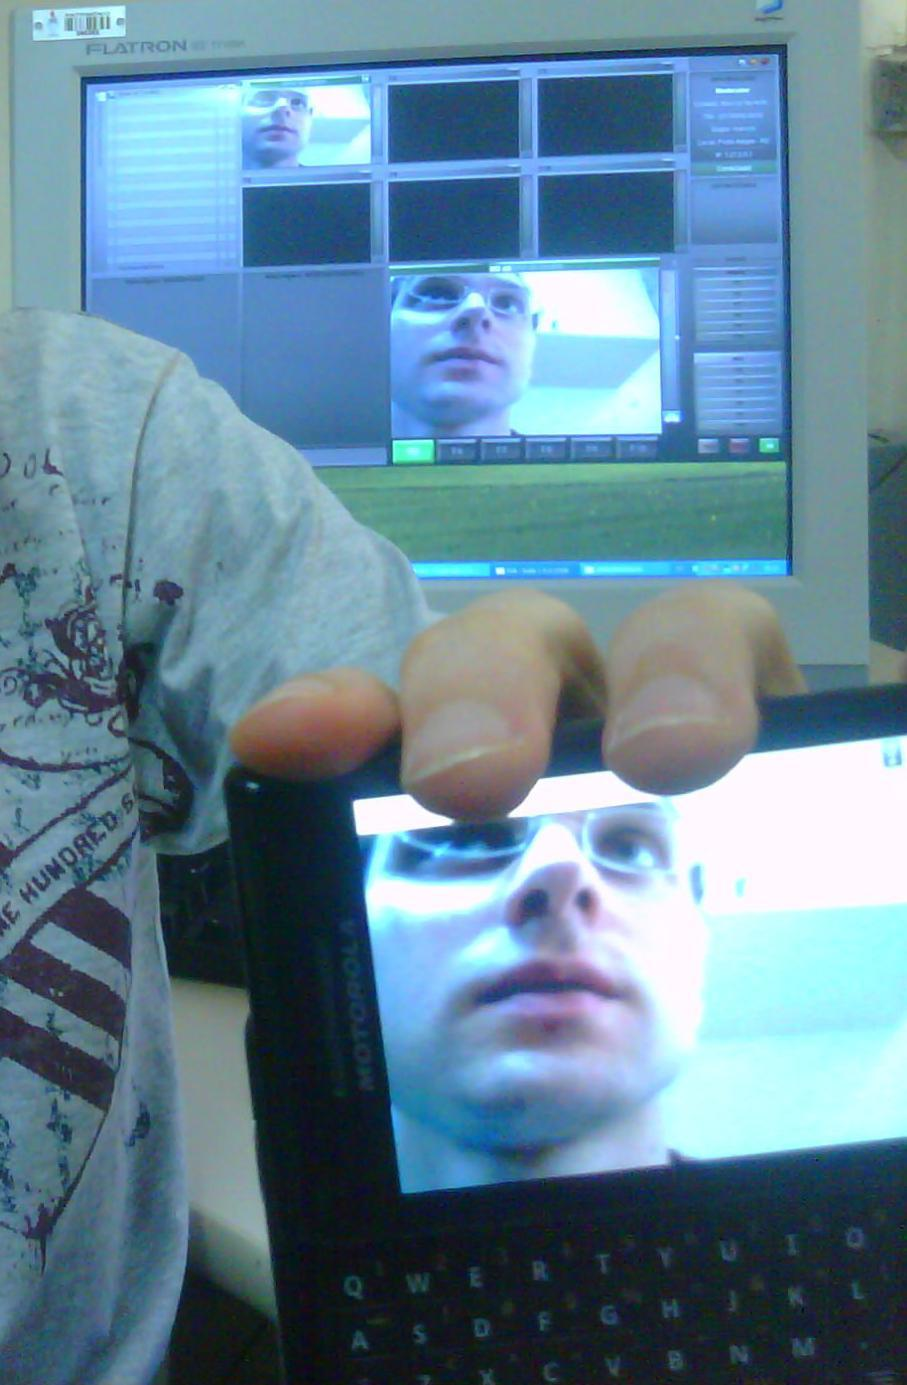
\includegraphics[scale=0.2]{./ivamobile.jpg}
 % ivamobile.jpg: 907x1385 pixel, 72dpi, 32.00x48.86 cm, bb=0 0 907 1385
\caption{Nossa estratégia integrada ao sistema IVA}
\end{figure}
\subsection{Teste 5}
Também integramos nossa estratégia a um outro sistema de videoconferências já existente chamado BigBlueButton, que funcionava apenas para desktops. Recebemos, no aplicativo Android, um fluxo de vídeo do BigBlueButton gerado por um desktop. O codec de vídeo utilizado foi FLV1 (também conhecido como Sorenson H.263), a uma resolução de 320x240. O vídeo foi exibido ampliado na máxima resolução no Samsung e no Motorola especificados na tabela~\ref{tabela_dispositivos} e também em um tablet rodando Android. O atraso ficou abaixo dos 400ms. \todo{inserir foto}.


\section{Conclusão}

\todo{escrever conclusão}

\section{Trabalhos futuros}

Estamos desenvolvendo um framework que irá encapsular todas as partes complexas da implementação dessa técnica. O framework permitirá que seja possível implementar aplicativos de interação por vídeo com a estratégia acima de modo simples e rápido, mas ao mesmo tempo oferecendo flexibilidade ao programador com relação a aspectos como, por exemplo, escolha dos codecs a serem utilizado e a escolha da forma de transmissão/recepção dos dados codificados. Por exemplo, o programador, se desejar, poderá implementar seu próprio protocolo para transmissão, utilizar um protocolo padrão já existente, ou utilizar a transmissão fornecida pelo framework. Também será possível utilizar o framework para arquivos de vídeo locais que estão codificados com codecs ou formatos não suportados em hardware pelo android, visto que o ffmpeg suporta, em software, um número muito grande de codecs.

%
% The following two commands are all you need in the
% initial runs of your .tex file to
% produce the bibliography for the citations in your paper.
\bibliographystyle{abbrv}
\bibliography{paper}  % sigproc.bib is the name of the Bibliography in this case
% You must have a proper ".bib" file
%  and remember to run:
% latex bibtex latex latex
% to resolve all references
%
% ACM needs 'a single self-contained file'!
%
\balancecolumns
% That's all folks!
\end{document}
